\begin{tcolorbox}[colback=violet!5!white, %
  colframe=violet!75!black, %
  title=\textbf{Parametric Nonlinear Optimization}]
  \textbf{General problem formulation of parametric programming:}
  \begin{align*}
    w^*(p)=\argmin_w \quad&f(w,p) \\
    \text{s.t.}\quad & g(w,p)=0 \\
    & h(w,p) \le 0
  \end{align*}
  With $y:=(w,\lambda,\mu)$, the KKT conditions can be re-stated as:
  \begin{align*}
    R_\text{A}(y,p)=
    \left[
    \begin{array}{c}
      \nabla_w \mathcal{L}(y,p) \\
      g(w,p) \\
      h_A(w,p) \\
      \mu_{\bar{\text{A}}}
    \end{array}
    \right] = 0,\quad h_{\bar{\text{A}}}(w,p) < 0,\quad \mu_\text{A} > 0
  \end{align*}
  For any neighbourhood of a given $\bar{p}$ and $w^*(\bar{p})$:
  ($y^*_\text{A}:=(w^*,\lambda^*, \mu^*_{\text{A}})$)
  \begin{align*}
    &\left.\underbrace{\left[\begin{array}{ccc}
            \nabla^2_{ww}\mathcal{L}&\nabla_w g&\nabla_w h \\
            \nabla_w g^\top& 0 & 0 \\
            \nabla_w h^\top& 0 & 0
          \end{array}\right]}_{\text{KKT-Matrix}}
                                 \frac{\partial y_\text{A}^*}{\partial p} +
                                 \frac{\partial}{\partial p}
                                 \left[
                                 \begin{array}{c}
                                   \nabla_w \mathcal{L} \\
                                   g \\
                                   h_\text{A}
                                 \end{array}
    \right]\right|_{p=\bar{p}} = 0,\\
    &\frac{\partial\mu^*_{\bar{\text{A}}}}{\partial p} = 0
  \end{align*}
  Predictor-Corrector-Algorithm (for inequ. constr. free problems):
  \begin{itemize}
  \item Start with initial values for $k_0, z_0, p_0$
  \item for $k=0,1,\dots$:
    \begin{itemize}
    \item Get new estimate $p_{k+1}$
    \item Generate new approx. solution $y_{k+1}$
    \end{itemize}

  \end{itemize}
  \begin{align*}
    y_{k+1}=y_k - 
    &\left(
    \frac{\partial R}{\partial y}(y_k, p_k)
    \right)^{-1} \\
    & \cdot
    \left(
      \underbrace{R(y_k, p_k)}_{\text{Correction-step (Newton)}} +
      \underbrace{\frac{\partial R}{\partial p}(y_k, p_k)(p_{k+1} - p_k)}_{\text{Tangential predictor}}
    \right)
  \end{align*}
  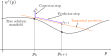
\includegraphics[width=0.8\textwidth]{pred_correct_alg}

  \textbf{IP method in online path following:}
  \begin{align}
    R_\tau(y,p) = 
    \left[
    \begin{array}{c}
      \nabla_w\mathcal{L}(y,p) \\ g(w,p) \\ h(w,p) + s \\ \mu_is_i - \tau
    \end{array}
    \right] = 0,\quad \mathrm{for\ a\ fixed\ }\tau > 0
  \end{align}
\end{tcolorbox}

%%% Local Variables:
%%% coding: utf-8
%%% mode: latex
%%% TeX-engine: xetex
%%% TeX-master: "../HelpSheet"
%%% End: